\documentclass{article}
\usepackage[T1]{fontenc} 
\usepackage[french]{babel}
\usepackage{graphicx}
\usepackage{enumitem}
\usepackage[a4paper,left=3cm,right=2cm,top=2.5cm,bottom=2.5cm]{geometry}

\begin{document}
\title{Projet Scientifique et Technique - Équipe Coc'Otter}
\author{Coc'Otter}
\date{2025}

\maketitle

\section{Présentation de l'équipe}

L'équipe Coc'Otter représente la convergence de deux histoires parallèles, celle de Rob'otter et de Cocobot, deux équipes composées d'anciens élèves de l'ENSEIRB. Nos membres ont tous fait leurs premiers pas en robotique au sein d'Eirbot, l'équipe officielle de l'école, une expérience qui a profondément marqué nos parcours professionnels et personnels. Cette fusion est née d'une volonté commune de poursuivre l'aventure de la coupe de robotique, tout en adaptant notre organisation aux contraintes de nos vies professionnelles et familiales.

\section{Mission et Objectifs}

Notre projet s'inscrit dans une vision à long terme de la robotique éducative et compétitive, avec une approche progressive et réaliste de nos objectifs.

\subsection{Transmission des connaissances post-COVID}
La période COVID a créé une rupture significative dans la chaîne de transmission des savoirs au sein des équipes de robotique étudiantes. Cette discontinuité s'est manifestée à plusieurs niveaux : perte de compétences techniques, affaiblissement des réseaux d'entraide, et diminution du nombre d'équipes actives. Face à ce constat, nous avons décidé de nous mobiliser pour reconstituer ce précieux écosystème d'échange de connaissances :

\begin{itemize}
    \item Nous maintenons une présence régulière dans les locaux d'Eirbot, créant ainsi des opportunités naturelles d'échange et de mentorat informel
    \item Nous participons activement à la reconstruction d'un réseau d'ingénieurs expérimentés, disponibles pour conseiller et guider les équipes étudiantes dans leurs projets
    \item Nous partageons notre expérience sur les aspects techniques complexes de la robotique
\end{itemize}

\subsection{Engagement dans la communauté}
Notre implication dans la communauté robotique va au-delà de la simple participation à la compétition. Plusieurs de nos membres contribuent activement au développement et à la pérennité de l'événement :
\begin{itemize}
    \item Un membre de notre équipe officient en tant qu'arbitre lors de le compétitions
    \item Un membre de l'équipe participe à la rédaction du règlements
    \item Tous nos développements sont systématiquement documentés et partagés en open-source, permettant à d'autres équipes de s'en inspirer ou de les améliorer
\end{itemize}

\subsection{Vision à Long Terme : Initiation des Jeunes à la Robotique}
Bien que notre focus pour l'édition 2025 soit principalement centré sur la stabilisation de notre équipe et la mise au point de nos robots, nous avons élaboré un projet pédagogique ambitieux pour les années à venir. Cette vision s'appuie sur notre expérience de parents et notre désir de transmettre notre passion :

\begin{itemize}
    \item Notre PAMI a été conçu avec une architecture permettant son évolution future vers une plateforme d'apprentissage
    \item L'intégration d'un joystick dans notre design actuel n'est pas qu'une facilité de debug : c'est la première étape d'une approche pédagogique inspirée des robots éducatifs populaires auprès des jeunes enfants (comme https://eu.robotshop.com/fr/products/ensemble-activite-souris-robotique-code-go)
    \item Nous prévoyons, dans les années à venir, de développer une interface de programmation visuelle basée sur Scratch, adaptée à l'apprentissage pour nos propres enfants (et leur camarades volontaires)
\end{itemize}


\section{Projet Technique}

\subsection{Le PAMI : Une Base Solide pour l'Avenir}

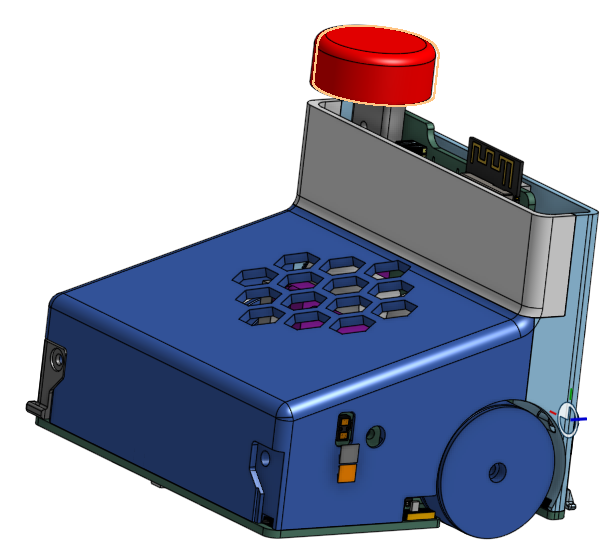
\includegraphics[width = 5cm]{pami_1}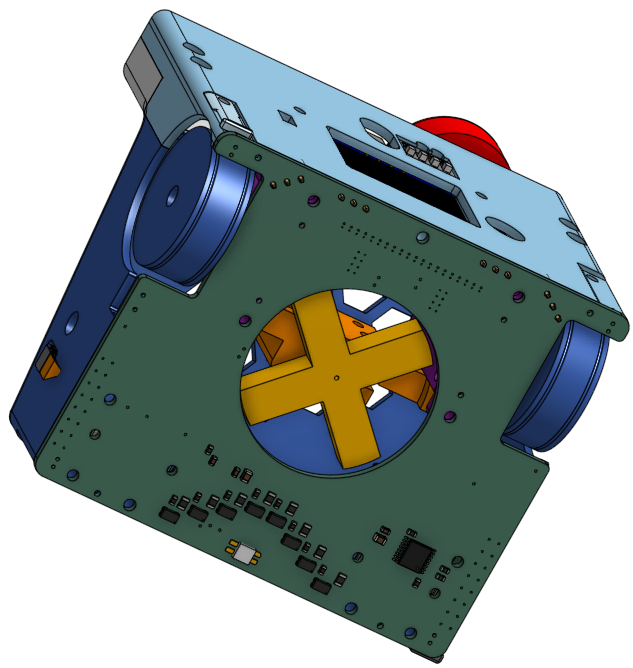
\includegraphics[width = 5cm]{pami_3}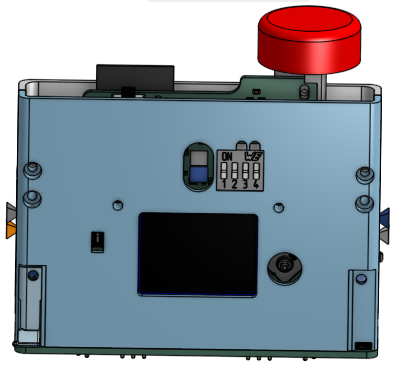
\includegraphics[width = 5cm]{pami_2}

Notre PAMI actuel représente la première étape d'une vision plus large. Sa conception répond aux exigences de la compétition tout en intégrant des éléments qui faciliteront son évolution future vers une plateforme pédagogique :


\begin{itemize}
    \item Ses dimensions compactes (85x73x65mm) et son poids optimisé (moins de 250g) le rendent manipulable et sécurisé pour de jeunes utilisateurs
    \item L'alimentation par cellule LiFePO4 unique simplifie la maintenance et la gestion de l'énergie
    \item L'architecture électronique repose sur deux PCB seulement, facilitant la compréhension de son fonctionnement
    \item L'utilisation de moteurs de drone avec réducteurs issus de servomoteurs offre un excellent rapport qualité-prix-performance
    \item Nos codeurs incrémentaux, entièrement conçus par nos soins, démontrent qu'il est possible de créer des solutions techniques avancées avec des moyens modestes
\end{itemize}

Les caractéristiques techniques actuelles incluent :
\begin{itemize}
    \item Des capteurs TOF pour le suivi de bordure et la détection d'obstacles, offrant une base solide pour l'apprentissage des concepts de perception robotique
    \item Un gyroscope pour la localisation précise, introduisant les notions de navigation et d'orientation
    \item Une programmation en Rust, choix qui reflète notre engagement pour la qualité et la fiabilité du code
\end{itemize}

Résumé de l'architecture:\\
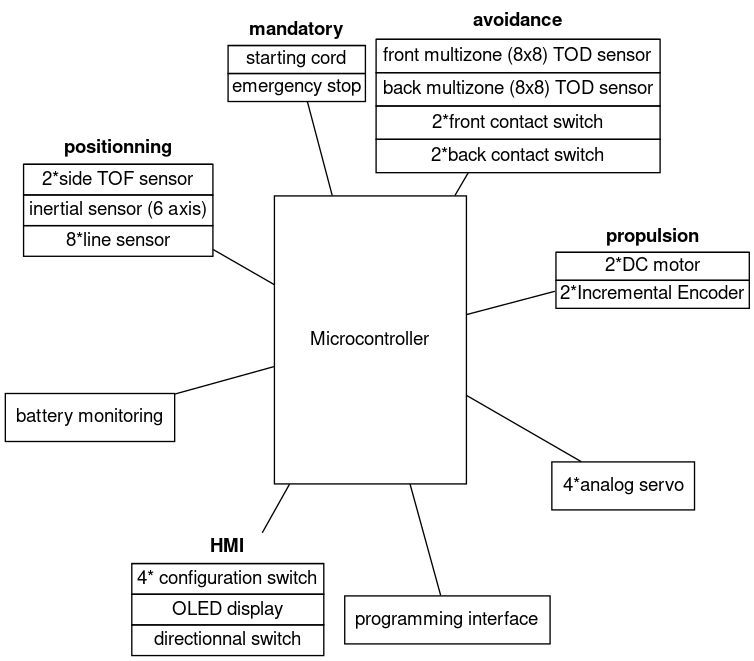
\includegraphics[width = 10cm]{projet_scientifique_technique_2025}

\section{Perspectives}

Notre approche est résolument progressive et réaliste. Pour l'édition 2025, nous nous concentrons sur les fondamentaux :
\begin{itemize}
    \item Stabilisation de notre équipe et de notre organisation
    \item Mise au point et fiabilisation de nos robots
    \item Établissement d'une présence régulière aux entraînements d'Eirbot
\end{itemize}

À moyen terme, nous prévoyons :
\begin{itemize}
    \item Le développement d'une interface de programmation visuelle (scratch, microsoft PXT) adaptée aux enfants
    \item L'implication grandissante de nos enfants dans le projet
    \item Et si le Planete Science le désire, la mise à disposition de nos robots pour des enfants du public lors de l'événement
\end{itemize}

\section{Communication et Partage}

Notre approche de la communication reflète notre philosophie d'ouverture et de partage :
\begin{itemize}
    \item Tous nos designs sont librement accessibles sur GitHub et OnShape, permettant à chacun de s'en inspirer ou de les améliorer
    \item Notre présence régulière aux sessions d'entraînement d'Eirbot crée des opportunités naturelles d'échange et d'apprentissage mutuel
\end{itemize}

\end{document}